\chapter{Locality Optimization of Record Layout}\label{methods}
\section{G-Store: Multilevel Partitioning}
    G-Store is a disk-based storage manager for graph data implemented and published by Steinhaus et al.~\autocite{steinhaus2010g}. 
    To the best of the author's knowledge, this is the first structured approach to improve locality in graph databases by altering records' placement into blocks.
    More specifically, to maximize performance, they try to place adjacent nodes close to each other to be read sequentially. 
    The rearrangement of the records is done when importing a new data set and is static after insertion.
    G-Store uses an adjacency list as the data structure and does not store these in an own file but directly next to the vertex in the same file.
    The broad schema of the placement method developed by Steinhaus et al.~\autocite{steinhaus2010g} is derived from multilevel partitioning methods described in Section~\ref{mlp}.
    Briefly, the multilevel partitioning algorithm works in three steps: coarsening, turn-around, and uncoarsening. 
    The coarsening phase tries to reduce the original graph to a smaller one that broadly preserves the underlying graph's structure. 
    A more expensive partitioning algorithm can then be applied to this smaller graph to solve the actual problem approximately and fast.
    During the uncoarsening, the approximate solution is refined, and the coarser graph is projected back until the original graph is mapped and restored.
    Finally, in the last step, the partitions are mapped to actual blocks.
    Note how similar the procedure is to the actual multilevel partitioning algorithm. 
    Thus we are more interested here in the differences from the reference algorithm.
    A broad overview of the method is shown in Figure~\ref{g-store}.
    
    \begin{figure}[htp]
        \begin{center}
            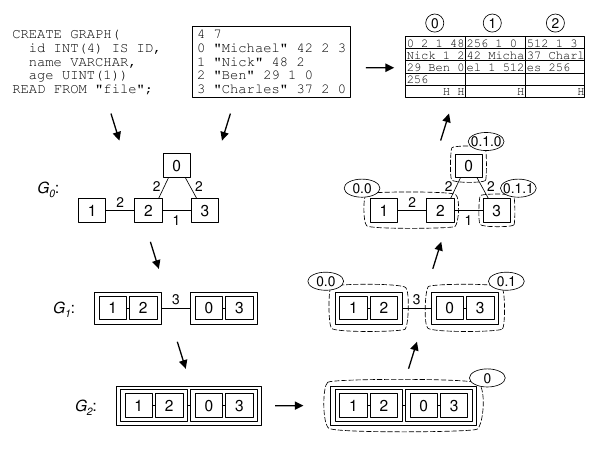
\includegraphics[keepaspectratio,width=0.7\textwidth]{img/06-rel_w/g-store.png}
        \end{center}
        \caption{A broad overview of the multilevel partitioning method applied by G-Store~\autocite{steinhaus2010g}.} 
        \label{g-store}
    \end{figure}

    
    In the next part of this section, we will use the notions of a finer and a coarser graph a lot. Let therefore $G = G_0 = (V_0, E_0)$ the original graph, and $G_i = (V_i, E_i)$ the graph that was coarsened $i$ times.
    
    \subsection*{Coarsening}
    The coarsening phase of G-Store's partitioning algorithm is called heavy edge matching (HEM) in Karypis formulation of the algorithm. 
    Thus the algorithm takes $G_i$ as an argument and returns $G_{i+1}$ along with a projection $Z_{i+1}$ specifying which finer nodes map to which coarser node.
    Coarsening proceeds in the original algorithm until a specific lower limit of vertices is reached.
    In the METIS implementation this is hard-coded to  $\max \left( 20k, 40 \log_2 k\right)$ where $k$ is a user defined parameter specifying the number of partitions.
    The algorithm used in G-Store keeps coarsening until there are no edges, i.e., only one vertex.
    Thus, it can be seen as a form of hierarchical agglomerative clustering~\autocite{hac} with the inverse edge weight acting as a distance function.
    
    Another modification is that in contrast to METIS~\autocite{karypis}, not only two edges are matched at a time but possibly many, and there is an upper limit to the vertex weights. 
    This depends on the coarsening factor $c(i) = \frac{|V_i| - |V_{i+1}|}{|V_i| - |\{v \in V | N_v = \emptyset \}|}$, with $i$ the level of coarsening, where $i=0$ it the original graph.
    The counter is the number of reduced vertices, and the denominator is the number of nodes in the larger graph minus the irreducible nodes.
    Initially, the allowed vertex weight $\theta$ is the size of a block.
    If this factor $c(i) < 0.3$ then the node weight $\theta$ is doubled as long as $\theta \leq 32$.
    Otherwise, the number of nodes that are allowed to be matched is incremented.
        
    \subsection*{Turn-Around}
    In G-Store, the turn-around assigns every vertex in the coarsest graph, whose weight is larger than a block's size, a distinct partition number.
    The other nodes are added up until their weight reaches the block's size and are assigned a partition number together.
    Thus the algorithm accepts a fully coarsened graph $G_i$ and returns the partition numbers for this graph $\phi_i$.
    
    This step is entirely different than in the reference multilevel partitioning algorithm.

    
    \subsection*{Uncoarsening}
    The uncoarsening phase consists of three different steps that are performed per level:
    projection, reordering, and refinement.
    Projection constructs the first mapping, reordering, swaps partitions, and refinement exchanges nodes between partitions.
    Each iteration of the entire uncoarsening procedure takes the coarser graph $G_{i+1}$ as an argument along with its the partition numbers $\phi_{i+1}$ and the mapping $Z_{i}$ and returns the one level uncoarsened graph $G_i$, along with the respective partition numbers $\phi_i$.
    The algorithm also defines a weight threshold per level. With $\overline{c}$ the average coarsening factor
    \[ \chi_i = \lfloor \frac{\text{block size}}{(1-\overline{c})^i} \rfloor. \]
    
    Further, it defines three objective functions:\\
    The first function is closesly related to the minimal linear arrangement problem~\autocite{lewis1983computers} and expresses that nodes that share an edge shall be minimally far appart from each other.
    \[ \min C_1 = \min \sum_{(u,v) \in E} |\phi(u) - \phi(v)| \]
    The second objective function aims to reduce the overall number of edges between the partitions.
    \[\min C_2 = \min \sum_{(u,v) \in E)} \begin{cases}
        1 & \phi(u) \neq \phi(v) \\
        0 & \text{ otherwise}
    \end{cases}
\]
    The last objective function penalizes the number of blocks that are linked. That is to reduce the number of overall linked blocks according to~\autocite{steinhaus2010g}.
    \[ \min C_3 = \min \sum_{i \leq j} 
    \begin{cases}
        1 & \phi(u) = i \wedge \phi(v) = j, \ (u,v) \in E \\
        0 & \text{ otherwise}
    \end{cases}
    \]
    
    Finally there are two functions that are similar to the first objective function that are used in the projection step called tension and modified tension:
    The tension is the weighted distance between the block of the vertices that share and edge. Let $v \in V_i$.
    \[ t(v) = \sum_{u \in N_v} w_{(u,v)} \phi_i(v) - \phi_i(u)\]
     The modified tension is just the same, but instead of using the actual graph, one uses the coarser graph $G_{i+1}$ and the projection $Z_{i}$ to estimate the tension:
     \[ t'(v) = \sum_{u \in N_v} w_{(u, v)} \phi_{i+1}(Z(v)) - \phi_{i+1}(Z(u)) \]
    
        \subsubsection*{Projection}
        This part of the algorithm constructs a first version of the finer-grained partition numbers $\phi_i$ from the coarser ones $\phi_{i + 1}$.
        The enumeration follows a Dewey numbering scheme~\autocite{dewey1894decimal}.
        That is, per level, one place in the partition label is added. 
        If the vertex $\phi_{i+1}(Z(v)) = 2$ and vertex $\phi_i(v) = 1$, then the overall partition label of the vertex is $2\text{.}1$. 
        
        Per partition in the coarser level graph, the algorithm either simply assigns the same partition number to all nodes $v_i \in Z(\phi{i+1,j})$ in the finer graph $G_i$ that were clustered into the respective coarser nodes, if the overall weight of the partition in the coarser graph is smaller than the weight threshold: $w_{\phi{i+1, j}} \leq \chi_i$.
        Otherwise the modified tension is computed for all nodes of the partition in the finer graph $\forall v_i \in Z(\phi{i+1,j}): t'(v_i)$.
        The minimal tension is extracted, placed to the leftmost free position in the partition, and the neighbors' tensions are updated. 
        This procedure is repeated until all nodes are placed.
        Each partition is marked with a flag.
	It is set when the partition was created from nodes in the right half of the coarser partition.
        
        The projection differs vastly from the reference algorithm that assigns the coarser partition number to all nodes in the finer-grained graph.
                
        \subsubsection*{Reordering}
        This step is non-existent in the multilevel partitioning algorithm.
        When swapping the above created partitions, only $C_1$ changes, but not $C_2$ or $C_3$. Using the just created flags, groups are identified which span two half coarser partitions $\phi_{i+1,j}, \phi_{i+1,j+1}$. Per group, the finer partitions are swapped as long as the overall absolute tension ($C_1$) decreases by some swap.
        In effect, this is a fix-point computation.
        
        \subsubsection*{Refinement}
        Finally, the refinement step tries to optimize a weighted sum of all the objective functions by moving vertices to other partitions.
        In the reference algorithm, this step uses the gain as defined in Section~\ref{kla}.
        Three used-defined parameters $\alpha, \beta, \gamma$ control the weighting. Another one specifies the number of iterations that shall be executed $r$.
        In each iteration, the algorithm steps over the partitions $\phi_{i,j}$ and creates a two dimensional array $A$ of dimension $|\phi_{i,j}| \times |P_{i,j}|$ with $P_{i,j} = \{ \phi_i(u) | v \in \phi_{i,j}, u \in N_n\} \setminus \phi_{i,j}$.
        Each entry is defined with $v$ the vertex that is to be moved to partition $k$:
        \[ a_{v,k} = \alpha C_1 + \beta C_2 + \gamma C_3 + \lambda \]
        Where $\lambda$ penalizes overfull blocks or rewards the filling of less filled blocks.


    
\section{ICBL: Diffusion Set-based Clustering}
    Ya\c{c}ar and Gedik propose another method to form and order blocks~\autocite{yacsar2015scalable, yacsar2017distributed}. 
        
    They define one metric for each of the task:
    \textit{Block locality} is defined by the means of conductance and cohesiveness. 
    Conductance is defined as the ratio of edge cuts to total edges in a block:
    \[ C_d (B) = \frac{|\{ (u,v) \in E: |\{u,v\} \cap V_B| = 1\}|}{|\{ (u,v) \in E: |\{u,v\} \cap V_B| > 0\}|} \]
    Cohesiveness is the number of nodes in the same blocks that are connected by an edge divided by the number of theoretically possible edges, i.e. $|V|^2$ in a directed graph. The authors assume an undirected self-loop free graph, thus the number of possible edges is $\frac{|V| (|V| - 1)}{2}$.
    \[ C_h (B) = \frac{|\{ (u,v) \in E: u,v \in V_B \}|}{|V|^2} \]
    As conductance takes edges between blocks into account and cohesiveness measures the edges within a block, they are complementary~\autocite{yacsar2015scalable}.
    Thus the locality of a block us defined as the geometric mean of the measures above, where the conductance is subtracted from one:
    \[ L(B) = \sqrt{C_h (B) \cdot (1 - C_d (B))} \]
    \textit{Ranking locality} is related to what we called tension before. 
    Here we do not measure it between partitions of the node but directly to the order's position. 
    Let $v \in V$ a node and $r(v)$ a function that assigns a natural number in the range of $\{0, \dots, |V|-1\}$ to each vertex.
    \[ R (v) = \sum_{u \in N_v} r(v) - r(u) \]
    The locality of a block is then defined by one minus the normalized average distance for all vertices in the block:
    \[ R(B) = 1 - \frac{1}{(|V| - 1)} \sum_{v \in V_B} \frac{R(v)}{|N_v|} \]
    
    \begin{figure}[htp]
        \begin{center}
            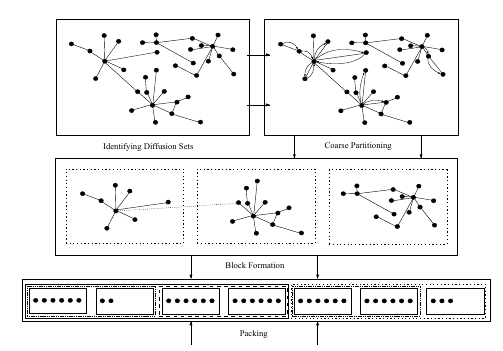
\includegraphics[keepaspectratio,width=0.8\textwidth]{img/06-rel_w/icbl.png}
        \end{center}
        \caption{A broad overview of the ICBL method by Ya\c{c}ar and Gedik~\autocite{yacsar2015scalable}.} 
        \label{icbl}
    \end{figure}

    ICBL is an acronym for the single steps performed by this algorithm. 
    It is designed to be implemented and executed using the map-reduce model.
    First, ICBL extracts so-called diffusion sets as features.
    Then it clusters the vertices based upon these features to split the graph into subgraphs.
    After that, it hierarchically clusters the subgraphs obtained in the previous step to form blocks.
    Finally, the just-formed blocks are ranked and laid out on disk.
    A visualization of the method is shown in Figure~\ref{icbl}.
    
    \subsection*{Identify Diffusion Sets}
    The diffusion set $\mathcal{D}_v$ of a vertex $v \in V$ is a characterization of the neighborhood of a vertex. 
    To identify the diffusion set, ICBL carries out $t$ random walks (Section~\ref{rand-w}, Algorithm~\ref{random_walk}) of length $l$.
    The authors characterize a random walk using the vertices, so from our definition, we need to extract the multiset of vertices from the walk.
    
    For choosing the parameters $t$ and $l$ Ya\c{c}ar and Gedik propose heuristics: 
    For $t$, construct the cumulative degree distribution $f(d) \mapsto P(x \leq d)$ and chose the minimal degree value such that the derivative of the cumulative degree distribution $f'(d) = 1$. The value of the derivative was derived empirically.
    Regarding $l$, the authors assume that the network exhibits the small world phenomenon~\autocite{kleinberg2000small}.
    In a network that has that property, the probability is high that there exists a path between any two nodes $u,v \in V$ of length $\ln{|V|}$.
    The random walk's length should not be too long as all nodes might be visitable. Thus the heuristic for choosing $l$ is $1 + \lceil \frac{\ln |V|}{k} \rceil$ where $k$ is the number of clusters in the next step.
    
    \subsection*{Coarse Clustering}
    After generating the diffusion sets, the graph is clustered using a variation of the k-Means algorithm~\autocite{lloyd1982least}. 
    It is used to partition the graph into $k$ smaller subgraphs, such that the computationally more expensive agglomerative hierarchical clustering~\autocite{hac} algorithm used in block formation can be executed in parallel.
    Instead of using a geometric distance function (like the Manhatten or the Euclidean distance between points on a plane), an alternated version of the Jaccard distance function~\autocite{jaccard1912distribution} is used. 
    The Jaccard function $J(u, v) = 1 - \frac{\mathcal{D}_u \cap \mathcal{D}_v}{\mathcal{D}_u \cup \mathcal{D}_v}$, i.e. the distance is the number of common elements divided by the set of all elements in both sets. 
    The altered distance is adjusted for multisets:  
    \[J_w (u, v) = 1 - \frac{\sum_{x \in \mathcal{D}_v \cap \mathcal{D}_u} \min (w_{\mathcal{D}_v}, w_{\mathcal{D}_u})}{\sum_{x \in \mathcal{D}_v \cup \mathcal{D}_u} \max (w_{\mathcal{D}_v}, w_{\mathcal{D}_u})} \]
    First, $k$ initial centers are chosen based upon the node degree and the distance to the already chosen centers.
    Then all nodes get assigned to the closest center. 
    Afterward, the centers are updated by building all diffusion sets' union and using the vertex with the highest weight as the new center.
    This is done until the centers do not change further.
    In order to determine the number of clusters, the authors propose a heuristic that is based on the available memory $M$ and the size of a vertex and the average diffusion set $s = \text{sizeof}(v) + \overline{\text{sizeof}(\mathcal{D})}$: 
    \[ k = \lceil \frac{s \cdot |V|}{\sqrt{0.8 \cdot M}} \rceil \]
    
    \subsection*{Block Formation}
    For each subgraph, agglomerative hierarchical clustering~\autocite{hac} is used to form blocks and label them for the ranking process.
    Each vertex starts in an own partition. 
    In every step the two closest partitions are merged. 
    The distance function here is the minimum of the previously defined weighted Jaccard distance of all nodes in the partition:
    \[ J_P (P_i, P_j) = \argmin_{u \in P_i, v \in P_j} J_w (\mathcal{D}_u, \mathcal{D}_v) \]
    Each partition maintains a label, that is used subsequently.
    In the beginning, the node id is used as a label. 
    When a potential merge would cause the so formed partition to exceed the block size, without one of the child partitions being already marked as a block, the partition is marked as a block.
    Additionally, the label is adjusted by appending a dot and a counter.
    If only one of the child partitions formed a block, the label of that partition is used.
    Finally, if both children formed a block before, their label is merged by inserting a double colon in between.
    The algorithm terminates when all partitions are assigned to a block.
    To keep track of the uncaptured nodes in a partition where one child formed a block before an additional field is necessary.    
    
    
    \subsection*{Layout}
    Finally, the tree is traversed to extract the formed blocks.
	These blocks are then sorted according to the label. 
    Next, each subgraph is treated as a vertex.
The distance between the two subgraphs is the inverse of the number of edges between them. Those with the lowest distance get merged, and the whole graph is laid out to disk.
    


\section*{Summary}
    In relational databases, the records are sorted to achieve locality~\autocite{ramakrishnan2000database, silberschatz1997database}. 
    Block formation is less of an issue there, as the sorting order of the records yields both the formation and the blocks' order.
    In contrast, graphs need to be partitioned into blocks, and if this is done, the sorting order is far from trivial.
    Both partitioning and linear arrangement are NP-complete problems~\autocite{lewis1983computers}.
    
     To summarize, previous methods first partitioned the graph by using an adapted version multilevel partitioning algorithm, combining feature extraction with traditional clustering algorithms~\autocite{overview_clust}, the Louvain method~\autocite{blondel2008fast} or the METIS implementation~\autocite{karypis} of the multilevel partitioning algorithm~\autocite{hendrickson1995multi}.
    Then based on the partitioning, the blocks were formed and ordered.
    In G-Store~\autocite{steinhaus2010g} this is done in the uncoarsening phase.
    In ICBL~\autocite{yacsar2017distributed, yacsar2015scalable}, hierarchical agglomerative clustering combined with a labeling scheme is used.
    Bondhu~\autocite{hoque2012disk} uses a scheme where the vertex with the highest partition is placed in the middle, and then iteratively, the neighbors with the highest edge weight are then placed next to it, and the two nodes are merged in the graph. 
    
    G-Store uses adjacency lists as a data structure.
    Thus the edges are placed directly next to the vertices in the very same file.
    For ICBL, the very same is true.
    They represent the graph using an adjacency list. 
    In the evaluation part of Ya\c{c}ar's and Gedik's work, the authors apply their order to Neo4J's incidence list structure~\autocite{Rodriguez2010ConstructionsFD, robinson2015graph}. 
    As already discussed in Section~\ref{n4j-rel}, the incidence list is implemented using an edge list with the incidence list included in the edge's record structure.
    To adapt ICBL's adjacency list to Neo4J, they insert the relations in the order of the adjacency list and store the nodes to their appearance in the edge list.    
    Regarding Bondhu\autocite{hoque2012disk}, the relationship arrangement is not mentioned in the paper.
    
    
\section{Incidence List Rearrangement}\label{\positionnumber}
    As the just inserted edges contain the incidence lists of the vertices, the order of these changed.
    If the edges are stored by insertion order, the incidence lists are sorted in a sense: 
    Edges that were inserted earlier also appear earlier in the incidence list and the other way around.
    Thus, reordering the incidence lists such that the first element in the list is also the first appearing relationship of that list in the underlying file will result in fewer jumps as shown in Table~\ref{inc-ord}.
    
    Consider the case in which we would reorganize the edges' position in the file but not reorder the incidence lists. 
    It is somewhat likely that relationships in the same block and the same incidence list are not accessed sequentially.
    Instead, many accesses to other elements are made in between that are potentially widely spread throughout the file.
    Depending on the node's degree (i.e., the length of the incidence list), the size of the graph, the buffer's capacity, and the number of queries that are concurrently executed, this might cause a lot of additional IOs.

